
\documentclass[aspectratio=169, handout]{beamer}

%\usepackage[table]{xcolor}
\mode<presentation> {
\setbeamercovered{transparent}
  \usetheme{Boadilla}

%  \usetheme{Pittsburgh}
%\usefonttheme[2]{sans}
\renewcommand{\familydefault}{cmss}
%\usepackage{lmodern}
%\usepackage[T1]{fontenc}
%\usepackage{palatino}
%\usepackage{cmbright}
 \usepackage{bm}
\useinnertheme{rectangles}
}
\usepackage{amsmath}
\setbeamercolor{normal text}{fg=black}
\setbeamercolor{structure}{fg= blue}
\definecolor{trial}{cmyk}{1,0,0, 0}
\definecolor{trial2}{cmyk}{0.00,0,1, 0}
\definecolor{darkgreen}{rgb}{0,.4, 0.1}
\usepackage{array}
\beamertemplatesolidbackgroundcolor{white}  \setbeamercolor{alerted
text}{fg=red}
\usepackage{tcolorbox}
\setbeamertemplate{caption}[numbered]\newcounter{mylastframe}

\font\domino=domino
\def\die#1{{\domino#1}}
\usepackage{tikz}
\usetikzlibrary{arrows}
\usepackage{colortbl}

\renewcommand{\familydefault}{cmss}
%\usepackage[all]{xy}

\usepackage{tikz}
\usepackage{lipsum}
\usetikzlibrary{angles,quotes}
 \newenvironment{changemargin}[3]{%
 \begin{list}{}{%
 \setlength{\topsep}{0pt}%
 \setlength{\leftmargin}{#1}%
 \setlength{\rightmargin}{#2}%
 \setlength{\topmargin}{#3}%
 \setlength{\listparindent}{\parindent}%
 \setlength{\itemindent}{\parindent}%
 \setlength{\parsep}{\parskip}%
 }%
\item[]}{\end{list}}
\usetikzlibrary{arrows}

\usecolortheme{lily}

\newtheorem{com}{Comment}
\newtheorem{lem} {Lemma}
\newtheorem{prop}{Proposition}
\newtheorem{condition}{Condition}
\newtheorem{thm}{Theorem}
\newtheorem{defn}{Definition}
\newtheorem{cor}{Corollary}
\newtheorem{obs}{Observation}
 \numberwithin{equation}{section}
 
\makeatletter
\def\beamerorig@set@color{%
  \pdfliteral{\current@color}%
  \aftergroup\reset@color
}
\def\beamerorig@reset@color{\pdfliteral{\current@color}}
\makeatother
\setbeamertemplate{navigation symbols}{}

\useoutertheme{miniframes}
\title[PLSC 30700]{Review of Linear Models Class 1-3}

\author{Robert Gulotty}
\institute[Chicago]{University of Chicago}
\vspace{0.3in}


\begin{document}


\begin{frame}
\maketitle
\end{frame}



\begin{frame}
\frametitle{Often the sample (co)variance appears in an alternative form:} 
\small{
\begin{align*}
\widehat{Var}(X)&=\frac{1}{N}\sum_i(x_i-\bar{x})(x_i-\bar{x}) \\
& =\frac{1}{N}\sum_i(x_i-\bar{x})x_i\\
 \widehat{Cov}(X,Y)&=\frac{1}{N}\sum_i(x_i-\bar{x})(y_i-\bar{y}) \\
& =\frac{1}{N}\sum_i(x_i-\bar{x})y_i\\
 \end{align*}}
\end{frame}

\begin{frame}
\frametitle{Algebra Demonstration} 
\small{
\begin{align*}
\widehat{Var}(X)&=\frac{1}{N}\sum_i(x_i-\bar{x})(x_i-\bar{x})  \pause \\
& =\frac{1}{N}\sum_ix_i^2-\bar{x}x_i-x_i\bar{x}+\bar{x}\bar{x}  \tag{Expand the square} \pause \\
& =\frac{1}{N}\sum_ix_i^2-\bar{x}\frac{1}{N}\sum_ix_i-\bar{x}\frac{1}{N}\sum_ix_i+\frac{1}{N}\sum_i\bar{x}\bar{x} \tag{Distribute the $\sum$} \\
& =\frac{1}{N}\sum_ix_i^2-\bar{x}\frac{1}{N}N\bar{x}-\bar{x}\frac{1}{N}\sum_ix_i+\bar{x}\bar{x} \tag{$\sum_i x_i=N\bar{x}$}\\
& =\frac{1}{N}\sum_ix_i^2-\bar{x}\frac{1}{N}\sum_ix_i \tag{$\bar{x}\bar{x}$ cancel}\\
& =\frac{1}{N}\sum_i(x_i-\bar{x})x_i\\
 \end{align*}}
\end{frame}

\begin{frame}
\begin{columns}
\begin{column}{0.5\textwidth}
  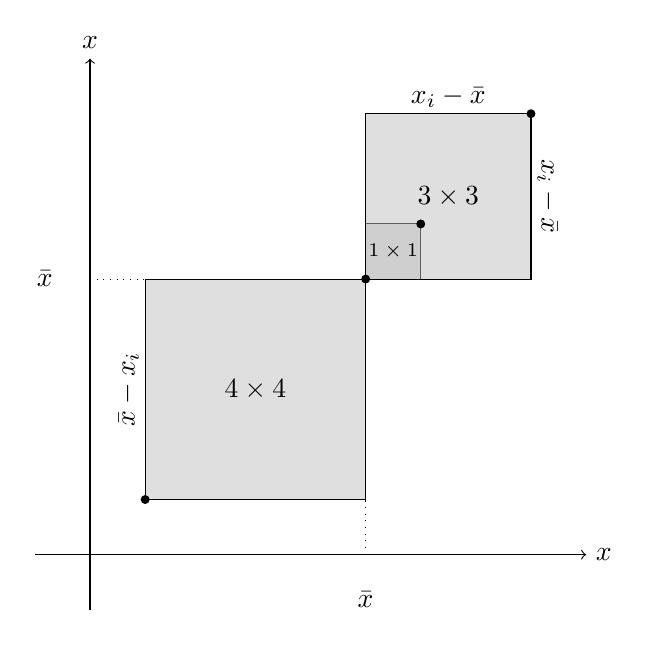
\begin{tikzpicture}[scale=.7]
    % Draw the squares and label their areas
    \foreach \x/\y in {1/1, 5/5, 6/6, 8/8}{
      \fill[gray!50,opacity=0.5] (\x,\y) rectangle ({5},{5});
      \draw (\x,\y) rectangle ({5},{5});
    }
      \node at (6.5,8.3) {$x_i - \bar{x}$};
    \node[rotate=-90] at (8.3,6.5) {$x_i - \bar{x}$};
    \node[rotate=90] at (.7,3) {$\bar{x}-x_i$};
    % Draw the rectangle at (5,5) and label its area
    % Draw the points
    \foreach \x/\y in {1/1, 5/5, 6/6, 8/8}{
      \filldraw[black] (\x,\y) circle (2pt);
    }
    % Draw the axes
    \draw[->] (-1,0) -- (9,0) node[right] {$x$};
    \draw[->] (0,-1) -- (0,9) node[above] {$x$};
    \draw[dotted] (5,0) -- (5,8);
    \node[below] at (5,-.5) {$\bar{x}$};
        \draw[dotted] (0,5) -- (8,5);
    \node[left] at (-.5, 5) {$\bar{x}$};
      \node at (3,3) {$4\times 4$};
        \node at (5.5,5.5) {\scriptsize{$1\times1$}};
          \node at (6.5,6.5) {$3\times 3$};
  \end{tikzpicture}
  \end{column}
  \begin{column}{0.5\textwidth}
 \begin{align*}
 \widehat{Var}(X)&=\frac{1}{N}\sum_i(x_i-\bar{x})(x_i-\bar{x})\\
 &=\frac{(-4*-4)+(1*1)+(3*3)}{4}\\
  &=\frac{26}{4}
 \end{align*} 
    \end{column}
  \end{columns}
\end{frame}


\begin{frame}
\begin{columns}
\begin{column}{0.5\textwidth}
  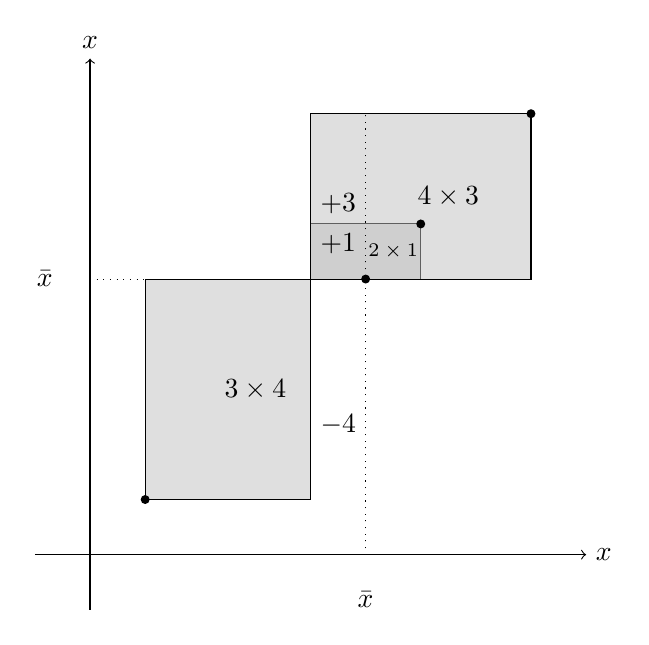
\begin{tikzpicture}[scale=.7]
    % Draw the squares and label their areas
    \foreach \x/\y in {1/1, 5/5, 6/6, 8/8}{
      \fill[gray!50,opacity=0.5] (\x,\y) rectangle ({4},{5});
      \draw (\x,\y) rectangle ({4},{5});
    }
    % Draw the rectangle at (5,5) and label its area
    % Draw the points
    \foreach \x/\y in {1/1, 5/5, 6/6, 8/8}{
      \filldraw[black] (\x,\y) circle (2pt);
    }
    % Draw the axes
    \draw[->] (-1,0) -- (9,0) node[right] {$x$};
    \draw[->] (0,-1) -- (0,9) node[above] {$x$};
    \draw[dotted] (5,0) -- node[near start, above left]{$-4$}  (5,8);
        \draw[dotted] (5,0) -- node[near end, above left]{$+3$}  (5,8);
  \draw[dotted] (5,0) -- node[near end, below left]{$+1$}  (5,8);
    \node[below] at (5,-.5) {$\bar{x}$};
        \draw[dotted] (0,5) -- (8,5);
    \node[left] at (-.5, 5) {$\bar{x}$};
      \node at (3,3) {$3\times 4$};
        \node at (5.5,5.5) {\scriptsize{$2\times1$}};
          \node at (6.5,6.5) {$4\times 3$};
  \end{tikzpicture}
  \end{column}
  \begin{column}{0.5\textwidth}
   \begin{align*}
 \widehat{Var}(X)&=\frac{1}{N}\sum_i(x_i-\bar{x})(x_i-(\bar{x}-1))\\
 &=\frac{(-4*-3)+(1*2)+(3*4)}{4}\\
  &=\frac{26}{4}
 \end{align*} 
    \end{column}
  \end{columns}
\end{frame}


\begin{frame}
\begin{columns}
\begin{column}{0.5\textwidth}
  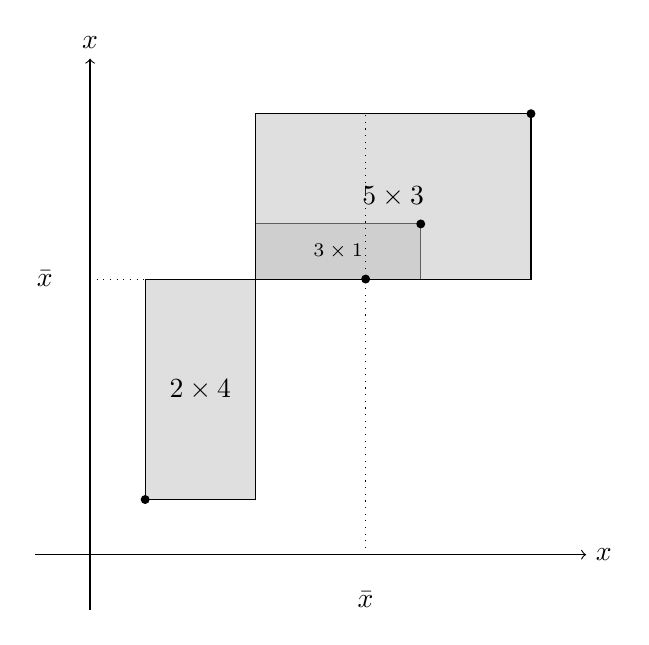
\begin{tikzpicture}[scale=.7]
    % Draw the squares and label their areas
    \foreach \x/\y in {1/1, 5/5, 6/6, 8/8}{
      \fill[gray!50,opacity=0.5] (\x,\y) rectangle ({3},{5});
      \draw (\x,\y) rectangle ({3},{5});
    }
    % Draw the rectangle at (5,5) and label its area
    % Draw the points
    \foreach \x/\y in {1/1, 5/5, 6/6, 8/8}{
      \filldraw[black] (\x,\y) circle (2pt);
    }
    % Draw the axes
    \draw[->] (-1,0) -- (9,0) node[right] {$x$};
    \draw[->] (0,-1) -- (0,9) node[above] {$x$};
    \draw[dotted] (5,0) -- (5,8);
    \node[below] at (5,-.5) {$\bar{x}$};
        \draw[dotted] (0,5) -- (8,5);
    \node[left] at (-.5, 5) {$\bar{x}$};
      \node at (2,3) {$2\times 4$};
        \node at (4.5,5.5) {\scriptsize{$3\times1$}};
          \node at (5.5,6.5) {$5\times 3$};
  \end{tikzpicture}
  \end{column}
  \begin{column}{0.5\textwidth}
   \begin{align*}
 \widehat{Var}(X)&=\frac{1}{N}\sum_i(x_i-\bar{x})(x_i-(\bar{x}-2))\\
 &=\frac{(-4*-2)+(1*3)+(3*5)}{4}\\
  &=\frac{26}{4}
 \end{align*} 

    \end{column}
  \end{columns}
\end{frame}


\begin{frame}
\begin{columns}
\begin{column}{0.5\textwidth}
  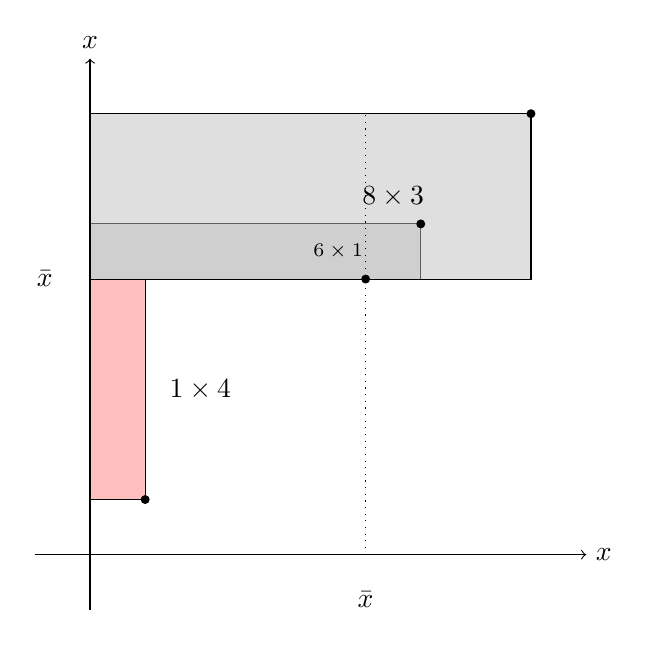
\begin{tikzpicture}[scale=.7]
    % Draw the squares and label their areas
    \foreach \x/\y in { 5/5, 6/6, 8/8}{
      \fill[gray!50,opacity=0.5] (\x,\y) rectangle ({0},{5});
      \draw (\x,\y) rectangle ({0},{5});
    }
    
      \fill[red!50,opacity=0.5] (1,1) rectangle ({0},{5});
      \draw (1,1) rectangle ({0},{5});
    
    % Draw the rectangle at (5,5) and label its area
    % Draw the points
    \foreach \x/\y in {1/1, 5/5, 6/6, 8/8}{
      \filldraw[black] (\x,\y) circle (2pt);
    }
    % Draw the axes
    \draw[->] (-1,0) -- (9,0) node[right] {$x$};
    \draw[->] (0,-1) -- (0,9) node[above] {$x$};
    \draw[dotted] (5,0) -- (5,8);
    \node[below] at (5,-.5) {$\bar{x}$};
        \draw[dotted] (0,5) -- (8,5);
    \node[left] at (-.5, 5) {$\bar{x}$};
      \node at (2,3) {$1\times 4$};
        \node at (4.5,5.5) {\scriptsize{$6\times1$}};
          \node at (5.5,6.5) {$8\times 3$};
  \end{tikzpicture}
  \end{column}
  \begin{column}{0.5\textwidth}
 \begin{align*}
 \widehat{Var}(X)&=\frac{1}{N}\sum_i(x_i-\bar{x})(x_i-(\bar{x}-\bar{x}))\\
 \widehat{Var}(X)&=\frac{1}{N}\sum_i(x_i-\bar{x})(x_i)\\
 &=\frac{(-4*1)+(1*6)+(3*8)}{4}\\
  &=\frac{26}{4}
 \end{align*} 

    \end{column}
  \end{columns}
\end{frame}

\begin{frame}
\frametitle{How does $y_k$ affect $Cov(X,Y)$?} 
\small{
\begin{align*}
 \widehat{Cov}(X,Y)&=\frac{1}{N}\sum_i(x_i-\bar{x})(y_i-\bar{y}) \\
 &=\frac{1}{N}\sum_i(x_i-\bar{x})(y_i-\frac{1}{N}\sum_j y_j) \pause \\ 
& =\frac{1}{N}\sum_i(x_i-\bar{x})y_i\\
 \end{align*}}
 
We can take the derivative with respect to $y_k$ in only one term of the summation.
\end{frame}




\begin{frame}
\frametitle{Geometry and the Dot product}
\begin{columns}
\begin{column}{0.3\textwidth}
  Suppose\\ $\bm{x}=(1,4)$, $\bar{x}=2.5$, $\bm{y}=(0,4)$, $\bar{y}=2$
  \begin{align*}
  (\bm{x}-\bar{x}\bm{1})\cdot(\bm{y})&=\\
-1.5*0+1.5*4&=6\\
(\bm{x}-\bar{x}\bm{1})\cdot(\bm{y}-\bar{y}\bm{1})&=\\
-1.5*(-2)+1.5*2&=6
\end{align*}
       \end{column}
  \begin{column}{0.7\textwidth}
  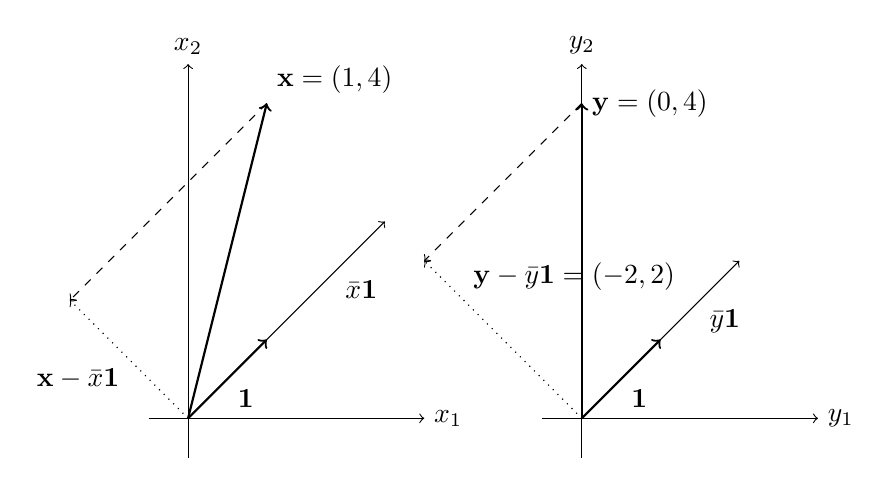
\begin{tikzpicture}
  % define the coordinates
  \coordinate (A) at (0, 0);
  \coordinate (B) at (1, 4);
  \coordinate (C) at (2.5, 2.5);
  \coordinate (D) at (-1.5, 1.5);
    \coordinate (E) at (1, 1);
  % draw the axis
        \draw[->] (-.5,0) -- (3,0) node[right] {$x_1$};
    \draw[->] (0,-.5) -- (0,4.5) node[above] {$x_2$};
    
  \draw[thick, ->] (A) -- node[at end, above right]{$\mathbf{x}=(1,4)$} (B);
   \draw[thick, ->] (A) -- node[midway, below right]{$\mathbf{1}$} (E);
  \draw[->] (A) -- node[near end, below right]{$\bar{x}\bm{1}$} +(C);
  \draw[dashed, ->] (B) -- (D);
  % draw the dotted line
  \draw[dotted,->] (A) --  node[midway, below left]{$\mathbf{x}-\bar{x}\bm{1}$}  (D);
  
  \coordinate (A) at (5, 0);
  \coordinate (B) at (5, 4);
  \coordinate (C) at (7, 2);
  \coordinate (D) at (3, 2);
    \coordinate (D1) at (3.5, 1.5);
    \coordinate (E) at (6, 1);
  % draw the vectors
          \draw[->] (4.5,0) -- (8,0) node[right] {$y_1$};
    \draw[->] (5,-.5) -- (5,4.5) node[above] {$y_2$};
  \draw[thick, ->] (A) -- node[at end, right ]{$\mathbf{y}=(0,4)$} (B);
     \draw[thick, ->] (A) -- node[midway, below right]{$\mathbf{1}$} (E);
    \draw[->] (A) -- node[near end, below right]{$\bar{y}\bm{1}$} (C);
  \draw[dotted,->] (A) --  node[near end, above right]{$\mathbf{y}-\bar{y}\bm{1}=(-2,2)$}  (D);
    \draw[dashed, ->] (B) -- (D);
\end{tikzpicture}
     \end{column}
  \end{columns}

\end{frame}


\begin{frame}
\frametitle{$\bm{a}\cdot \bm{b}=||\bm{a}||||\bm{b}||\cos\theta$}
\begin{columns}
\begin{column}{0.4\textwidth}

  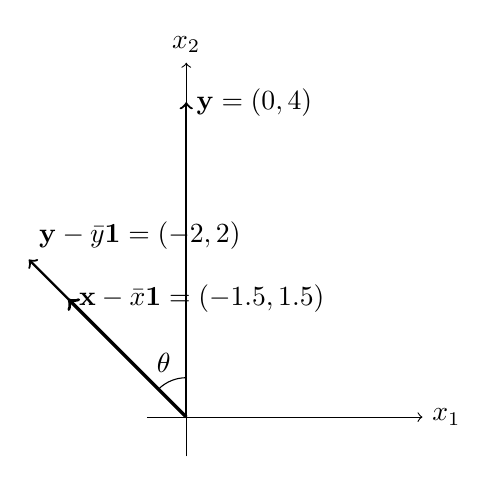
\begin{tikzpicture}
  % define the coordinates
  \coordinate (A) at (0, 0);
  \coordinate (B) at (0, 4);
  \coordinate (C) at (2, 2);
  \coordinate (D) at (-2, 2);
    \coordinate (D1) at (-1.5, 1.5);
    \coordinate (E) at (1, 1);
  % draw the axis
      \draw[->] (-.5,0) -- (3,0) node[right] {$x_1$};
    \draw[->] (0,-.5) -- (0,4.5) node[above] {$x_2$};
      % draw the vectors
  \draw[thick,->] (A) -- node[at end, right ]{$\mathbf{y}=(0,4)$} (B);
    \draw[very thick,->] (A) --  node[at end, right]{$\mathbf{x}-\bar{x}\bm{1}=(-1.5,1.5)$}  (D1);
  \draw[thick, ->] (A) --  node[at end, above right]{$\mathbf{y}-\bar{y}\bm{1}=(-2,2)$}  (D);
  \draw pic[draw=black, angle radius=5mm, angle eccentricity=1.5, "$\theta$"] {angle = B--A--D1};
\end{tikzpicture}\\
\end{column}
\begin{column}{0.6\textwidth}

Note, $\bm{y}-\bar{y}\bm{1}\perp\bar{y}\bm{1}$, so $[(0,4)-(0,0)-(-2,2)]$ is a right triangle and cos $\theta = \frac{\text{Adjacent}}{\text{Hypotenuse}}$
$$||\bm{y}-\bar{y}\bm{1}||=||\bm{y}||\cos\theta$$
Any vector minus its means lies on a hyperplane $\perp\bm{1}$ and so are parallel to one another ($\theta=0\text{ or }\pi$)
\begin{align*}
\bm{y}-\bar{y}\bm{1}\parallel \bm{x}-\bar{x}\bm{1} 
\rightarrow \cos (0)=1\rightarrow\\
||\bm{x}-\bar{x}\bm{1}||||\bm{y}||\cos(\theta)&=\\
 \sqrt{4.5}\sqrt{16}*cos(\pi/4)&=6\\
||\bm{x}-\bar{x}\bm{1}||||\bm{y}-\bar{y}\bm{1}||\cos(\theta)&=\\
\sqrt{4.5}*\sqrt{8}\cos(0)&=6
\end{align*}
\end{column}
\end{columns}
 \end{frame}

\end{document}
